\documentclass[12pt,a4paper]{article}
\usepackage[margin=2cm,bottom=2cm]{geometry}
\usepackage[utf8]{inputenc}
\usepackage{hyperref}
\usepackage{graphicx}
\usepackage[table]{xcolor}
%page anchorlar gerekirse alt satırı sil
\hypersetup{pageanchor=false}


\begin{document}
\begin{titlepage}
 \centering
 
\includegraphics[scale=0.3]{bilgi_logo}\\
 {\scshape\LARGE Istanbul Bilgi University\\}
 \vspace{1cm}
 {\scshape\Large Laureate Bilgi Robotic Competition\\}
 \vspace{2cm}
 {\huge\bfseries BASTION THE SENTINEL\\}
 {\scshape\Large Park Cleaner Robot\\}
 \vspace{2cm}
 {\Large\itshape Ömer Faruk Bakırcı\\}
 {\Large\itshape Tolga Akdemir\\}
 {\Large\itshape Şeyhmus Okan Pordoğan\\}
 {\Large\itshape Furkan Karakoyunlu\\}
 \vspace{4cm}
 {\Large\itshape Supervisor\\Eray Baran}
 \vfill
 \vfill
 {\large \today\\}
 \href{http://www.bastionthesentinel.com}{www.bastionthesentinel.com}
\end{titlepage}


% Table of contents
\tableofcontents
\pagebreak

\section{Scope}
 \begin{flushleft}
  In today's era consuming is essential for human beings. This ``consuming" leads to wastes which is a danger for mother nature. 
  it leaves great amount of damage 
  to the nature. Thus, there is huge space to fill for recycling 
  and \textbf{Bastion The Sentinel} will help to close the gap. We are aiming for people to not waste their time for garbage 
  collecting and separating for recycling from the beginning. The purpose of creating this robot is reducing manpower in 
  collecting garbage and increase recycling to make future better.
  \begin{figure}[h]
   \begin{center}
    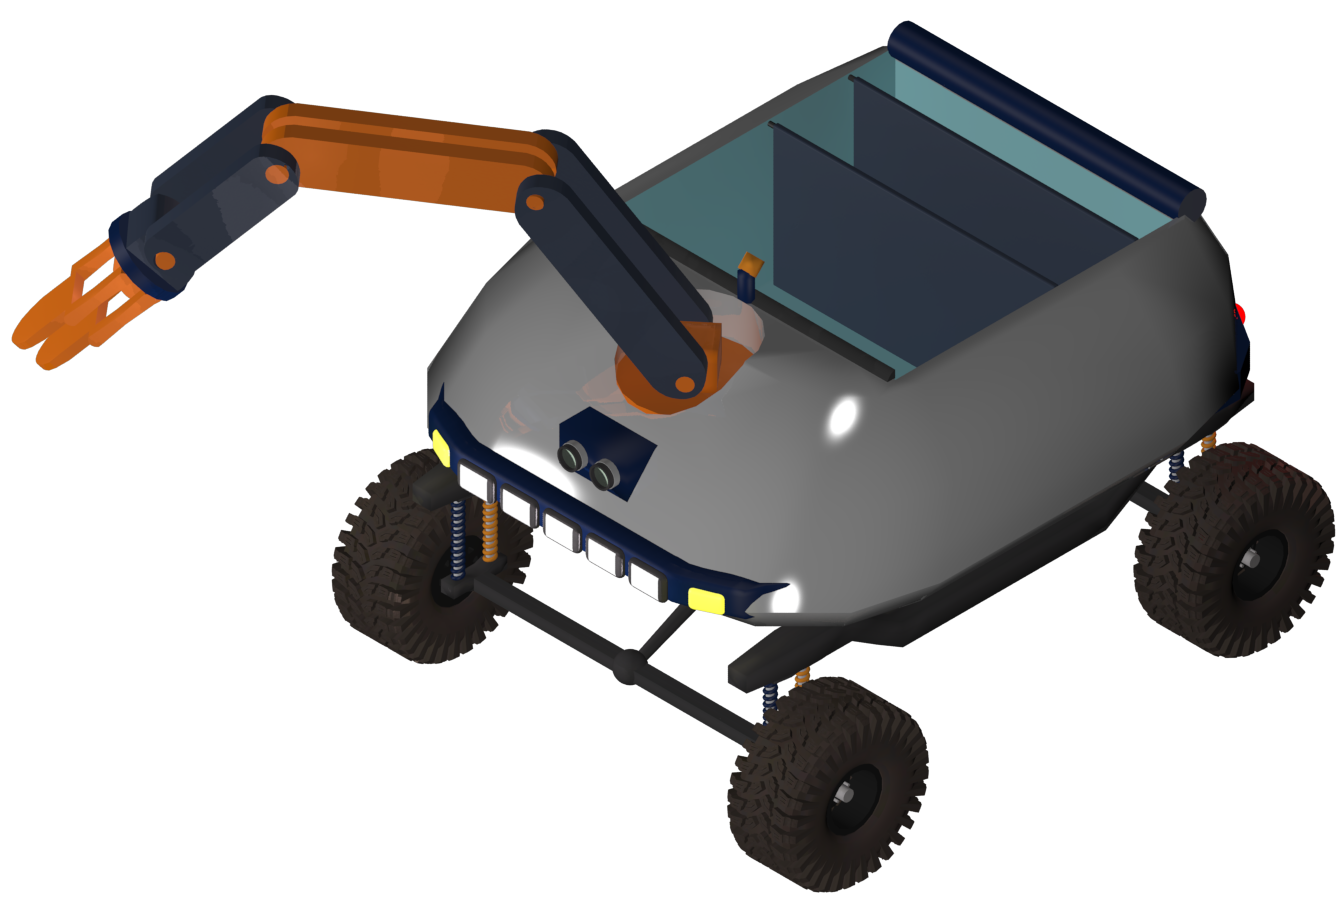
\includegraphics[scale=0.2]{perspective_box_open}
    \caption{Perspective capture of the \textbf{Bastion The Sentinel}}
   \end{center}
  \end{figure}
 \end{flushleft}
  
\section{Device Functionality}
 \begin{flushleft}
  \textbf{Bastion The Sentinel} is designed as a semi-autonomous robot. It will be a multi-tasking robot and it has two 
  main parts. First part is movement controls and the second part is collecting garbages via image-processing. In addition to 
  image processing abilities it can also be controlled by an operator. In the image processing part first it will consider color, 
  if it is not successful it will perform image processing for the shape ofkm the object. It will separate 
  all of the garbage by particularly and put them into box which is placed on top of the robot. After that operator will do separation.  
  If there are one or more objects to collect, operator can change the box's volume and decide the count of separators.
  There could be obstacles around or unfavorable weather conditions like rain, snow, etc. Therefore some incidents are 
  inevitable. Because of this top of the box can be closable. \\
  For increasing the maneuver ability, we placed steering wheels to the back, besides we choose to place impulse to the front of 
  the robot. The reason for choosing this method is while its collecting the garbages on the back, it will increase the weight because 
  of that giving impulse in front will be more reasonable. \\
  Another significant thing is deciding the sensors. We will use a proximity sensor for our robot. This way it will 
  understand if its approaching to an object or not. In addition to proximity sensor we will use depth sensor for calculating the depth. 
 \end{flushleft}
 
 \pagebreak
 \section{Overall Design Scheme}
 \begin{flushleft}
  The block diagram which represents the overall system design is shown below\\
  \begin{figure}[h]
   \begin{center}
    \includegraphics[scale=0.5]{block_diagram}
    \caption{Block diagram of the system}
   \end{center}
  \end{figure}
  The overall system of \textbf{Bastion The Sentinel} consists of 4 main blocks: input block, controller block, 
  communication block and output block.
 \end{flushleft}
 
 \section{Details of Design}
  
   \subsection{Input Block}
    \begin{flushleft}
     \textbf{Bastion The Sentinel} will collect data from environment via its sensors and cameras. These data will be used to 
     feed micro controllers. The main points are:
     \begin{itemize}
      \item \textbf{Bastion The Sentinel}'s robotic arm divided by three joints and has one gripper.
      \item Robotic arm can rotate 360$^{\circ}$ and it can be collapsed to minimize the area. Also the gripper part will 
      have the ability to rotate up to 180$^{\circ}$.
      \item Garbage detection is reinforced by proximity sensor. It will provide information about whether there is an object around 
      of the robot.
      \item Depth sensor will be used to verify incoming data's from proximity sensor. If they match the robotic arm will start the 
      collecting process.
     \end{itemize}

    \end{flushleft}

    \subsubsection{Cameras}
     \begin{flushleft}
      Visual information will be taken from the (CMOS Camera Sensor)cameras. The robot has led lights which allows it to 
      operate in the dark. Video informations will be taken from 3 different cameras, 2 of them will be placed 
      in front and the other one will be placed on the back facing to box. We will use front cameras as depth sensors and vision 
      cameras. They will have two mods and we can switch from one to another. Cameras will be connected to Raspberry Pi 3 and 
      video information will be processed on the user side for performance issues.
     \end{flushleft}
     
   \subsection{Control Block}
    \begin{flushleft}
     \begin{figure}[h!]
      \begin{center}
       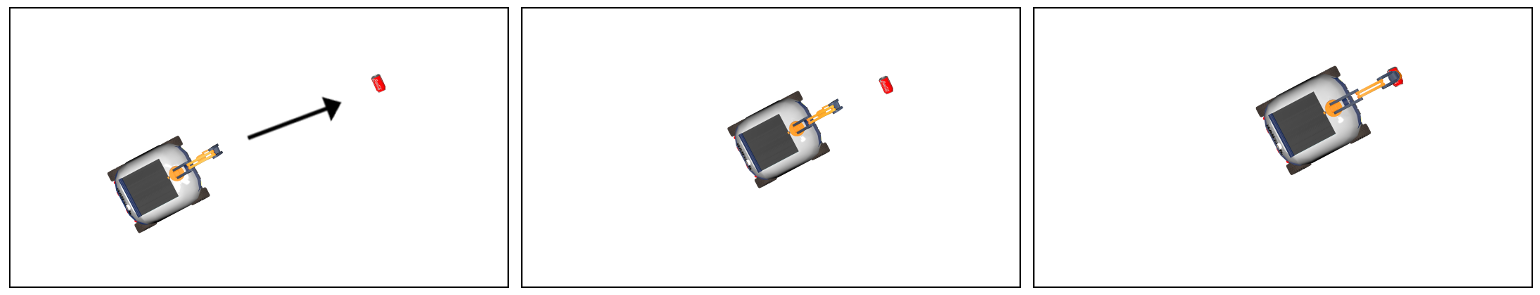
\includegraphics[scale=0.3]{3frame}
       \caption{\textbf{Bastion The Sentinel} is approaching to an object.}
      \end{center}
     \end{figure}
     In this block, Arduino (and Raspberry Pi) will manage the wheel system. It gives impulse to front wheels while it only 
     rotates from back wheels. Two motor shields will drive four wheels.
    \end{flushleft}

   \subsection{Output Block}
    \begin{flushleft}
     Micro controllers empower the DC motors for movement process on front wheels and also it empowers servo motors for 
     rotating back wheels. After the data has been collected from the environment, micro controllers uses the robotic arm 
     to gather objects to its container. All this information will be shared with the operator.\\
     \textbf{Bastion The Sentinel} can use artificial intelligence to determine and separate the objects.\\
     \bigskip
     \begin{figure}[h]
      \begin{center}
       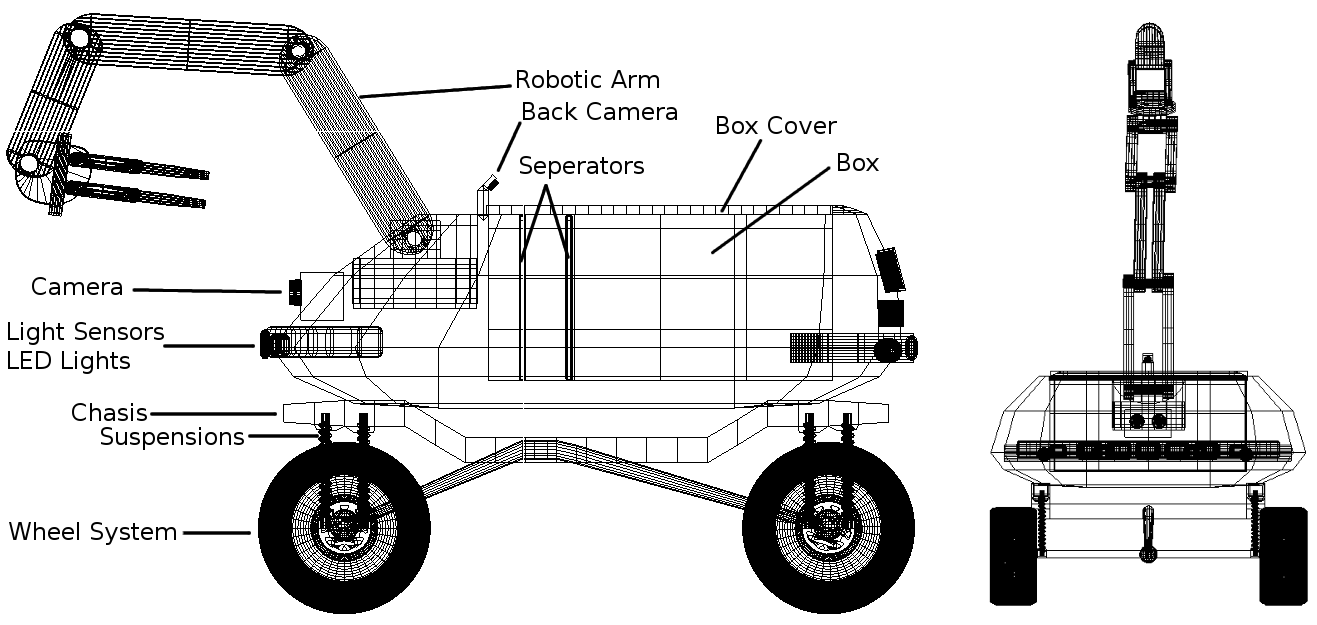
\includegraphics[scale=0.4]{skeleton_detailed}
       \caption{Mechanical design details (Side view and front view)}
      \end{center}
     \end{figure}
     \bigskip
    \end{flushleft}

   \subsection{Communication Block}
    \begin{flushleft}
     The communication will be provided via wireless connection which is on the Rasbperry Pi 3. Sensor 
     information will be processed on the robot and will be sent to user. However, video data will be processed on 
     the user side because of the efficiency. Our main goal is to provide simultaneous video transmission to grab 
     objects in the best accurate way. We will be able to communicate with the cameras by Raspberry Pi 3's WiFi.
    \end{flushleft}
 
 \pagebreak
 
 \section{Time Table and Work Schedule}
  \begin{flushleft}
   \begin{figure}[h!]
   \begin{center}
    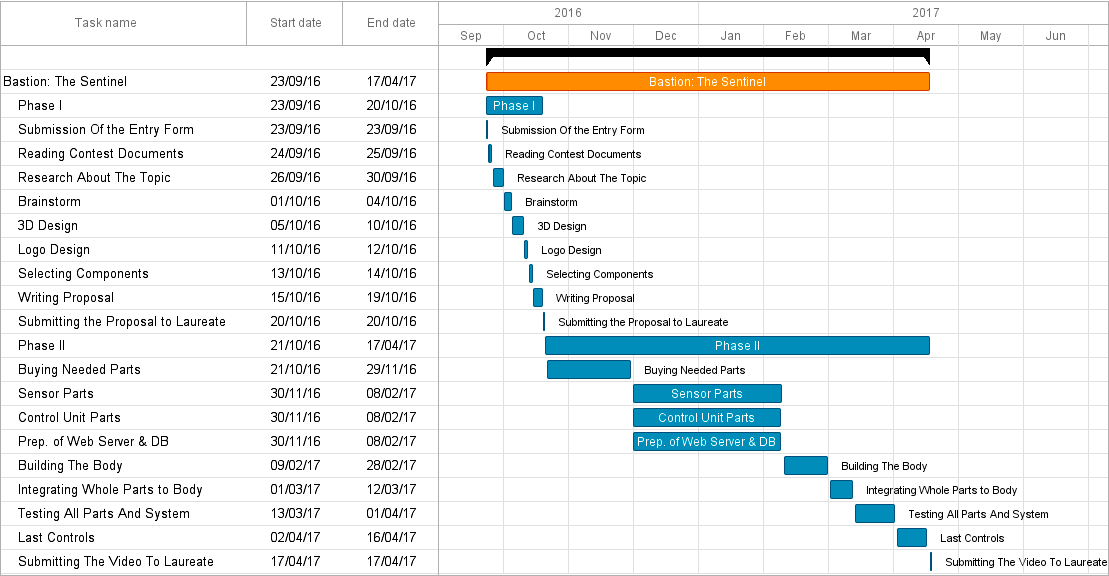
\includegraphics[scale=0.4]{time_schedule}
    \caption{Time table and work schedule}
   \end{center}
  \end{figure}
  \end{flushleft}
  
 \section{CAD Design and Device Dimensions}
  \begin{flushleft}
   \begin{figure}[h!]
   \begin{center}
    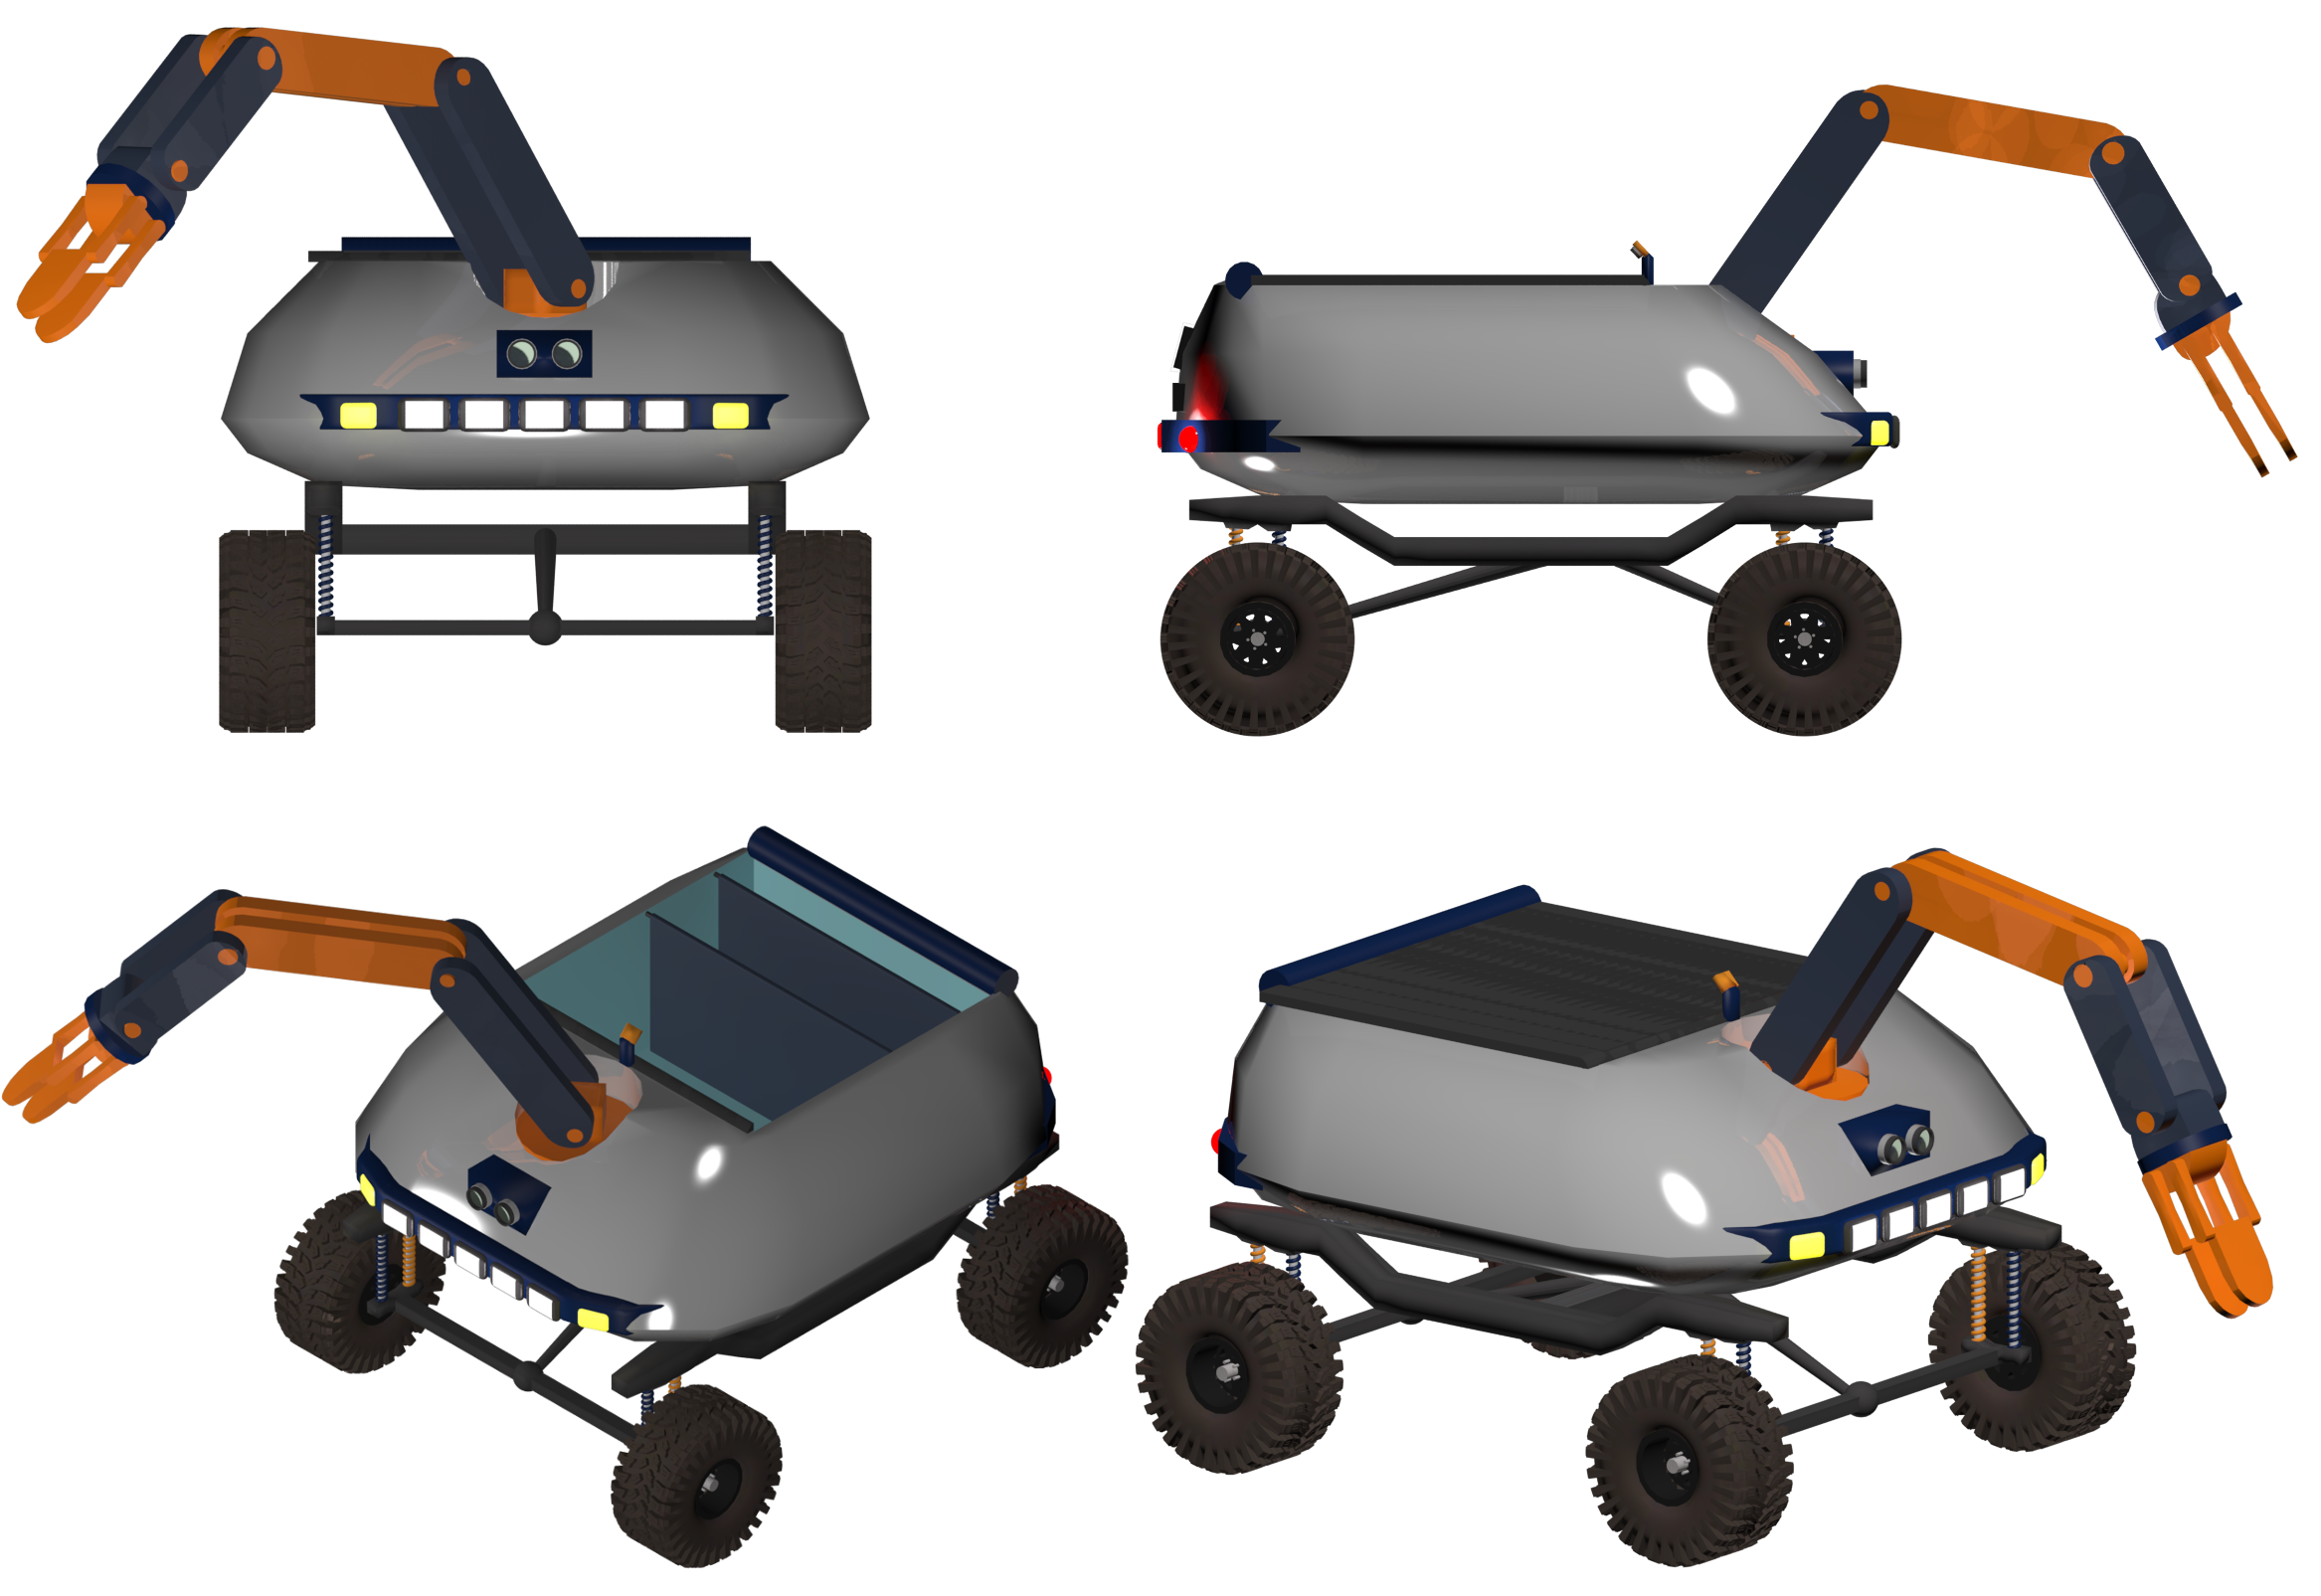
\includegraphics[scale=0.2]{cad_design}
    \caption{CAD design, Approximate Dimensions: Length=50cm Width=45cm Height=40cm}
   \end{center}
  \end{figure}
  \end{flushleft}

 \section{Budget}
  \subsection{Budget Breakdown}
  \begin{flushleft}
  \begin{center}
   % colors of the tabular
   \definecolor{Gray}{gray}{0.95}
   \definecolor{LightCyan}{rgb}{0.88,1,1}
   \definecolor{LightGreen}{rgb}{0.88,0.9,0.9}
   
   \newcolumntype{g}{>{\columncolor{Gray}}c}
   
   \begin{tabular}{ |c|g|c|g|c| }
    \hline
    \rowcolor{LightGreen}
    \multicolumn{5}{ |c| }{Materials}                                    \\
    \hline
    \rowcolor{LightCyan}
    Number &   Material Name   & Quantity & Unit Price (\$) & Total Cost(\$) \\
    \hline
           & DC Motor          & 2        & \$30            & \$60       \\
    \hline
           & Servo Motor       & 6        & \$8             & \$48       \\
    \hline
           & Wheel             & 4        & \$15            & \$60       \\
    \hline 
           & Bearing Hub       & 4        & \$12            & \$48       \\
    \hline
           & Carbon Fiber Chassis  & 1    & \$60            & \$60       \\
    \hline
           & Upper Plexy Body  & 1        & \$45            & \$45       \\
    \hline
           & Robotic Arm Components & 1   & \$250           & \$250      \\
    \hline
           & Shock Absorber    & 8        & \$15            & \$120      \\
    \hline
    \rowcolor{LightGreen}
    \multicolumn{5}{ |c| }{Kits}                                         \\
    \hline
    \rowcolor{LightCyan}
    -&   Kit Name        & Quantity & Unit Price (\$) & Total Cost(\$)   \\
    \hline
     & Raspberry Pi3 Maxi & 1        & \$150            & \$150          \\
    \hline
     & Arduino Mega Rev3 & 1        & \$40            & \$40             \\
    \hline
     & Arduino Motor Shield & 2     & \$15            & \$30             \\
    \hline
    \rowcolor{LightGreen}
    \multicolumn{5}{ |c| }{Sensors}                                      \\
    \hline
    \rowcolor{LightCyan}
    -&   Sensor Name        & Quantity & Unit Price (\$) & Total Cost(\$)  \\
    \hline
    & Proximity Sensor      & 1        & **            &           \\
    \hline
    & Light Sensor      & 1        & **            &           \\
    \hline
    & CMOS Camera Sensor & 3       & \$40          & \$120           \\
    \hline
    \rowcolor{LightGreen}
    \multicolumn{5}{ |c| }{Communication and Internet}                 \\
    \hline
    \rowcolor{LightCyan}
    -&   Name        & Quantity & Unit Price (\$) & Total Cost(\$)  \\
    \hline
    & Wireless       & 1        & **              &                    \\
    \hline
    & Domain Name    & 1        & \$25            & \$25            \\
    \hline
    & Web expenses   & 1        & \$30            & \$30            \\
    \hline
   \end{tabular}
   \\ 
   \footnotesize \textit{** indicates that Raspberry Pi 3 Maxi Kit includes this sensor }\normalsize
  \end{center}
  \end{flushleft}

  \subsection{Total Budget}
   \begin{flushleft}
    The prices for the components of the \textbf{Bastion The Sentinel} are shown in the table.
    \begin{itemize}
     \item Base price: \$1086
     \item Worst case scenario: \$500
     \item Total: \$1586
    \end{itemize}
   \end{flushleft}

  
 \section{Safety and Environmental Sustainability}
  \begin{flushleft}
   \textbf{Bastion The Sentinel} operates in a semi-autonomous way. It has a robotic arm and can interact 
   with objects in environment. However, there can be living creatures or objects that we do not want to 
   interact with. This situation creates a safety and security issues. Using the robot with an operator 
   will be safest way to avoid these type of situations. 
  \end{flushleft}

 \section{Business Plan}
 \begin{flushleft}
  In Turkey, pollution rates are higher than other European countries. There are many researches for solving 
  this problem. Yet there is not a proper way to solve it, however, our robot is the most convenient 
  way to reduce the pollution problem. The purpose of creating this robot is to protect the nature and 
  speed up the recycling process. It takes so many years for some materials to dissolve in nature. Also \%75 of 
  garbages are recyclable but \%30 percent of it used used in recycling process. Moreover, if you leave recycling to nature, 
  it will take years, that's why we thought that someone should step up and do something about it.
 \end{flushleft}
\end{document}
